\documentclass[problem]{mcs}

\begin{pcomments}
  \pcomment{CP_a_baseball_series}
  \pcomment{from: S09.cp12r}
\end{pcomments}

\pkeywords{
  probability
}

%%%%%%%%%%%%%%%%%%%%%%%%%%%%%%%%%%%%%%%%%%%%%%%%%%%%%%%%%%%%%%%%%%%%%
% Problem starts here
%%%%%%%%%%%%%%%%%%%%%%%%%%%%%%%%%%%%%%%%%%%%%%%%%%%%%%%%%%%%%%%%%%%%%

% F09, S09

\begin{problem}
{\bf [A Baseball Series]} \\
The New York Yankees and the Boston Red Sox are playing a
two-out-of-three series.  (In other words, they play until one team
has won two games.  Then that team is declared the overall winner and
the series ends.)  Assume that the Red Sox win each game with
probability $3/5$, regardless of the outcomes of previous games.

Answer the questions below using the four step method.  You can use
the same tree diagram for all three problems.

\bparts

\ppart What is the probability that a total of 3 games are played?

\ppart What is the probability that the winner of the series loses the
first game?

\ppart What is the probability that the \textit{correct} team wins the
series?

\eparts

\begin{solution}
A tree diagram is worked out below.
%
\begin{center}
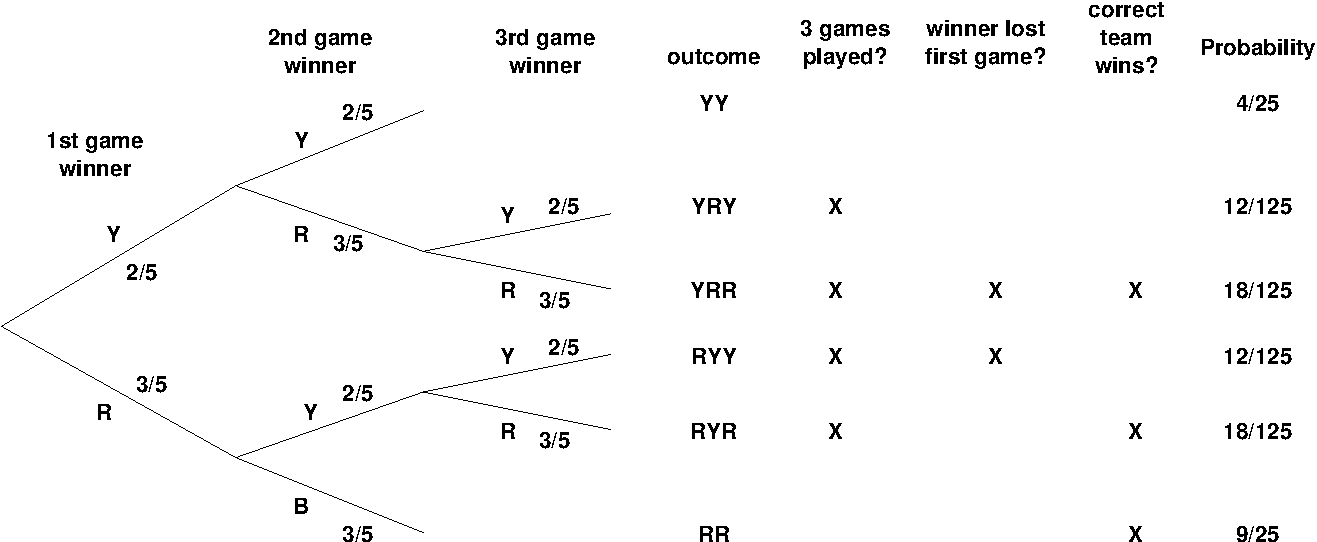
\includegraphics[width=6.25in]{figures/series.pdf}
\end{center}
%
From the tree diagram, we get:
%
\begin{align*}
\pr{\text{3 games played}}
    & = \frac{12}{125} + \frac{18}{125} + \frac{12}{125} + \frac{18}{125}
      = \frac{12}{25} \\
\pr{\text{winner lost first game}}
    & = \frac{18}{125} + \frac{12}{125}
      = \frac{6}{25} \\
\pr{\text{correct team wins}}
    & = \frac{18}{125} + \frac{18}{125} + \frac{9}{25} = \frac{81}{125}
\end{align*}

\end{solution}

\end{problem}

%%%%%%%%%%%%%%%%%%%%%%%%%%%%%%%%%%%%%%%%%%%%%%%%%%%%%%%%%%%%%%%%%%%%%
% Problem ends here
%%%%%%%%%%%%%%%%%%%%%%%%%%%%%%%%%%%%%%%%%%%%%%%%%%%%%%%%%%%%%%%%%%%%%

\endinput